\documentclass{article}
\usepackage[utf8]{inputenc}
\usepackage[english]{babel}


\usepackage{amsthm}
\newtheorem{theorem}{Theorem}
\newtheorem{proposition}{Proposition}
\newtheorem{definition}{Definition}
\usepackage{subfigure}
\usepackage{float}
\usepackage{lineno,hyperref}
\modulolinenumbers[5]
\usepackage{amssymb}
\usepackage{amsmath}
\usepackage{mdwtab}
\usepackage{url}
\usepackage{multirow}
\usepackage{float}
\usepackage{graphicx}
\graphicspath{{./figure/}}
\usepackage{fancyhdr}    % for headers and footers
\usepackage{hyperref}
\usepackage{xcolor}
\usepackage{tikz}
\usepackage{lipsum}
\usepackage{listings}
\usepackage{newtxtext,newtxmath}
\usepackage{ tipa } % for \textchi

\usepackage{mathtools}
\usepackage{setspace}
\usepackage{booktabs}
\usepackage{amssymb}
\usepackage{multirow}
\usepackage{array}
\usepackage{makecell}


%\usepackage{amsthm} % For Theorem, proof, Defintion for details see http://latextutorials.co.uk/documentation/theorems-and-definitions/
\usepackage[linesnumbered,ruled]{algorithm2e}
\usepackage{multicol}
\usepackage[margin=2.5cm]{geometry}
\usepackage{geometry} % Set page layout
\geometry{a4paper, margin=1in} % A4 page layout with 1-inch margin

\usepackage{setspace} % Line spacing package
\onehalfspacing % Set line spacing to 1.5

% \usepackage{titlesec} % Custom title, headings, and sub-headings
% \titleformat{\title}{\bfseries\fontsize{16}{20}\selectfont}{\thesection}{1em}{} % Title style: Bold, size 16
% \titleformat{\section}{\bfseries\fontsize{14}{17}\selectfont}{\thesection}{1em}{} % Heading style: Bold, size 14
% \titleformat{\subsection}{\bfseries\fontsize{12}{15}\selectfont}{\thesubsection}{1em}{} % Sub-heading style: Bold, size 12

% \usepackage{caption} % Custom figure captions
% \captionsetup{font=footnotesize, labelfont=bf, justification=centering} % Caption style: Size 10, center alignment

\setlength{\parskip}{12pt} % Set space before and after paragraphs

\begin{document}

%For Algorithm

\newcolumntype{L}[1]{>{\raggedright\let\newline\\\arraybackslash\hspace{0pt}}m{#1}}
\newcolumntype{C}[1]{>{\centering\let\newline\\\arraybackslash\hspace{0pt}}m{#1}}
\newcolumntype{R}[1]{>{\raggedleft\let\newline\\\arraybackslash\hspace{0pt}}m{#1}}


\title{}
\author{}
%\date{February 2021}
\date{}

% Title page 
\newcommand*{\titleGP}{\begingroup % Create the command for including the title page in the document
	\centering % Center all text
	\vspace*{\baselineskip} % White space at the top of the page
	
	\rule{\textwidth}{1.6pt}\vspace*{-\baselineskip}\vspace*{2pt} % Thick horizontal line
	\rule{\textwidth}{0.4pt}\\[\baselineskip] % Thin horizontal line
	{\LARGE HAMMING CODE IMPLEMENTATION} \\
	
	\rule{\textwidth}{0.4pt}\vspace*{-\baselineskip}\vspace{3.2pt} % Thin horizontal line
	\rule{\textwidth}{1.6pt}\\[\baselineskip] % Thick horizontal line
	
	\scshape % Small caps
	
	\vspace*{1\baselineskip} % Whitespace between location/year and editors
	{\large{\textsl{
				{A \\ 
					Synopsis Report \\ %\underline{•}
					Submitted in Partial Fulfillment of the Bangalore University\\
					for the Degree \\ 
					of\\
					\large \bf Bachelor of Technology \\
                    in\\
                    \large \bf Electronics and \\
                    \large \bf Communication Engineering 
	}}}}\\
	[5ex] \emph{by} \\[1ex]
	%Submitted by \\[\baselineskip]
    
	{\large 
    {
    \begin {enumerate}
    \item \centering { \bf Meghana G N}\\\\U03NM21T043041 VI SEM, B.Tech,
     \item { \bf Meghashyama N Aithal}\\U03NM21T043042 VI SEM, B.Tech,
    \item { \bf Mohammed Daanish Hassain}\\U03NM21T043043 VI SEM, B.Tech,
    \item   \bf Mohammed Hamza}\\U03NM21T043044 VI SEM, B.Tech,
    \end{enumerate} 
 \\ \par} % Editor list\\ {\tt your.email@iitx.ac.in}}\\[2cm] % Editor affiliation
	
	Under the supervision of \\ % Tagline(s) or further description
	%[\baselineskip] % Tagline(s) or further description
	\large Dr. Harsha MV\\ \\
 	\vfill % Whitespace between name and publisher logo
    \vspace*{\baselineskip}
	
\includegraphics[scale=0.2]{logo2.jpeg}\\
	\vfill
 
% 	{\scshape  \today} \\[0.3\baselineskip] % Year published
	{Department of Electronics and Communication Engineering}\\
	{\large Universtiy of Vivesvaraya College of Engineering}\par % Publisher
 \thispagestyle{empty} 

	\endgroup}


\maketitle
	%\pagestyle{empty} % Removes page numbers
        \vspace{-2.5cm}
\titleGP % This command includes the title page
    
\clearpage
	
	

\lhead{\emph{Contents}} % Set the left side page header to "Contents"
\tableofcontents
	\thispagestyle{empty}
	%\include{abstract/abstract}
	\cleardoublepage
	\typeout{}

% Line gap
\setstretch{1.2}

\pagenumbering{arabic} 

% % -------------------------------
% % ABSTRACT
% % -------------------------------

% \begin{abstract}
% \noindent
% \lipsum[1-2]
   
     
% \end{abstract}


% -------------------------------
% INTRODUCTION
% -------------------------------
\section{Introduction}
The Hamming Code is an error-detecting and error-correcting code used in telecommunications, computer systems, and data storage. It was developed in the late 1940s by Richard W. Hamming, an American mathematician and computer scientist, while working at Bell Labs. Hamming was frustrated with the frequent errors in data transmission and storage, particularly in early computer systems, which often required manual error correction. To address this, he devised a mathematical method that could automatically detect and correct errors, leading to the development of the Hamming Code.
\cite{6772729}



% -------------------------------
% Background INFO
% -------------------------------
\subsection{Background Information}
The Hamming Code is based on binary linear error-correcting codes and is particularly known for its ability to detect and correct single-bit errors in transmitted data. It uses redundant bits, known as parity bits, to create a code that can check for errors and identify which bit is incorrect if an error is detected. The original Hamming Code (referred to as (7,4) Hamming Code) uses seven bits, where four are data bits, and three are parity bits.

The code operates using a method called Hamming Distance, which is the number of bit positions in which two code words differ. For error detection and correction, the Hamming Code relies on a minimum Hamming Distance of three between any two code words, allowing it to detect up to two-bit errors and correct one-bit errors.\\
\textbf{Key Principles}
    \begin{enumerate}
        \item \textbf{Parity Bit Calculation}: \\ Parity bits are added at specific positions in the code word. Each parity bit covers a certain set of data bits and ensures that the number of 1s in that subset is even (even parity) or odd (odd parity).
        \item \textbf{Error Detection and Correction}: \\ When a code word is received, parity checks are performed. If the parity doesn’t match, it indicates an error, and the position of the error can be determined using a binary index derived from the parity checks.
    \end{enumerate}

% -------------------------------
% Background INFO
% -------------------------------
\subsection{Current Trends and Application}
While technology has evolved significantly since the Hamming Code's invention, it remains a foundational concept in digital error correction. Its simplicity and efficiency in correcting single-bit errors make it popular in applications where minimal redundancy and simplicity are key. Some modern applications and trends include:
    \begin{enumerate}
        \item \textbf{Low-Power, Embedded Systems}: \\ : The Hamming Code is used in memory systems like static RAM (SRAM) in low-power devices, such as IoT devices and sensors, where power efficiency and low data redundancy are crucial.
        \item \textbf{Network Communications}: \\ Although advanced codes like LDPC (Low-Density Parity-Check) codes and Turbo Codes are more common in modern high-speed networks, the Hamming Code’s simplicity still makes it useful for error detection in simpler protocols and small-scale networks.
    \end{enumerate}
    

% Methodology 
\section{Literature Survey}
A 15-bit Hamming Code, such as (15,11) Hamming Code, was used to encode 11 data bits into 15 bits by adding four parity bits. This allows for single-bit error correction and double-bit error detection. Implementing the Hamming code encoding and correction between two communicating Micro controller.\cite{10.11648/j.pamj.20160506.17}




\subsection {Mathematical principles}
\begin{theorem}[Hamming code]
\label{hamming code}
Hamming codes are a class of binary linear code. For each integer \[r \geq 2 \] there is a code-word with block length
\[n=2*r - 1\]\\
message length 
\[k=2*r-r-1\]
\end{theorem}

\begin{figure*}[!ht]
    \centering
    
    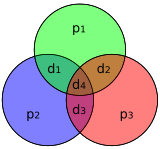
\includegraphics[width=7cm, height=4cm, keepaspectratio]{figures/Hamming(7,4).png}      
    
    \caption{The Hamming(7,4) code (with r = 3)}
    \label{fig:fig1}
\end{figure*}


\subsection{Implementation Steps}
\begin{itemize}

\item {Software implementation}

Writing program to encode data into hamming code and decode the same. The program is ran and in the due process random bit flips in data is forced which is corrected using hamming code and hence making data Error Free.

\item {Implementation between two communicating Arduino}

Establishing Reliable Communication link between two Arduinos. of which one playing the role of a transmitter and 

\item {Hardware Implementation}

Designing the the logic block diagram of hamming encoder on and Decoder and realizing the same using logic ICs and connecting them 
\end{itemize}


   

\section{OBJECTIVE-I : Understanding and Designing the Hamming Code Algorithm}
\subsection{Code Layout}
\begin{itemize}
\item Encode 8-bit data into a 12-bit code word.
\item Compute parity bits to ensure error detection and correction.
\item Include error detection and single-bit error correction for the receiving Arduino.
\item \textbf{Bit positions: }
\end{itemize}
The 12-bit Hamming code is structured as follows:

    \begin{table}[h!]
        \centering
        \caption{Hamming (12,8) Code Layout}
        \begin{tabular}{|c|c|c|c|c|c|c|c|c|c|c|c|c|}
            \hline
            \textbf{Bit Position} & 12 & 11 & 10 & 9 & 8 & 7 & 6 & 5 & 4 & 3 & 2 & 1 \\
            \hline
            \textbf{Bit Type} & D8 & D7 & D6 & D5 & P8 & D4 & D3 & D2 & P4 & D1 & P2 & P1 \\
            \hline
        \end{tabular}
        
    \end{table}
     D1 to D8 are the 8 data bits.\\
     P1, P2, P4, and P8 are the 4 parity bits. 

\subsection{Designing the Hamming Code}
\begin{itemize}

\item {Step 1: Determine the number of parity bits.}
Given a data bit sequence of length \(m\), the number of parity bits \(r\) is determined such that:
\begin{equation}
2^r \geq m + r + 1
\end{equation}

\item  {Step 2: Position the parity bits}
Place the parity bits at positions that are powers of 2 (i.e., positions 1, 2, 4, 8, etc.). The remaining positions are reserved for data bits.

\item {Step 3: Calculate parity bit values,}
The value of each parity bit is calculated based on specific bits in the data sequence. For each parity bit, cover bits are determined using binary representation. For example, parity bit \(P_1\) covers bits at positions where the least significant bit of their binary representation is 1.

\textbf{Example}
Consider a 4-bit data sequence: \texttt{1011}.

\begin{enumerate}
    \item Calculate the number of parity bits needed:
    \begin{equation}
    2^r \geq 4 + r + 1 \implies r = 3
    \end{equation}
    \item Insert parity bits at positions 1, 2, and 4: \texttt{P1, P2, 1, P4, 0, 1, 1}.
    \item Calculate values for each parity bit:
    \begin{itemize}
        \item \(P_1\) covers positions 1, 3, 5, 7.
        \item \(P_2\) covers positions 2, 3, 6, 7.
        \item \(P_4\) covers positions 4, 5, 6, 7.
    \end{itemize}
\end{enumerate}






A (12,8) Hamming code uses 8 data bits and 4 parity bits to form a 12-bit code word. The parity bits are strategically placed in positions that are powers of two (1, 2, 4, and 8), while the data bits are placed in the remaining positions.\cite{khadir}
\end{itemize}


\section{OBJECTIVE-II : Implementing on software}

\textbf{Arduino Sketch for Hamming Code}

Below is a simple Arduino sketch to implement a Hamming code encoding and decoding algorithm:\cite{beneater2018}


\begin{tabular}{cc}

\textbf{Encoding Algorithm} & \textbf{Decoding Algorithm} \\

       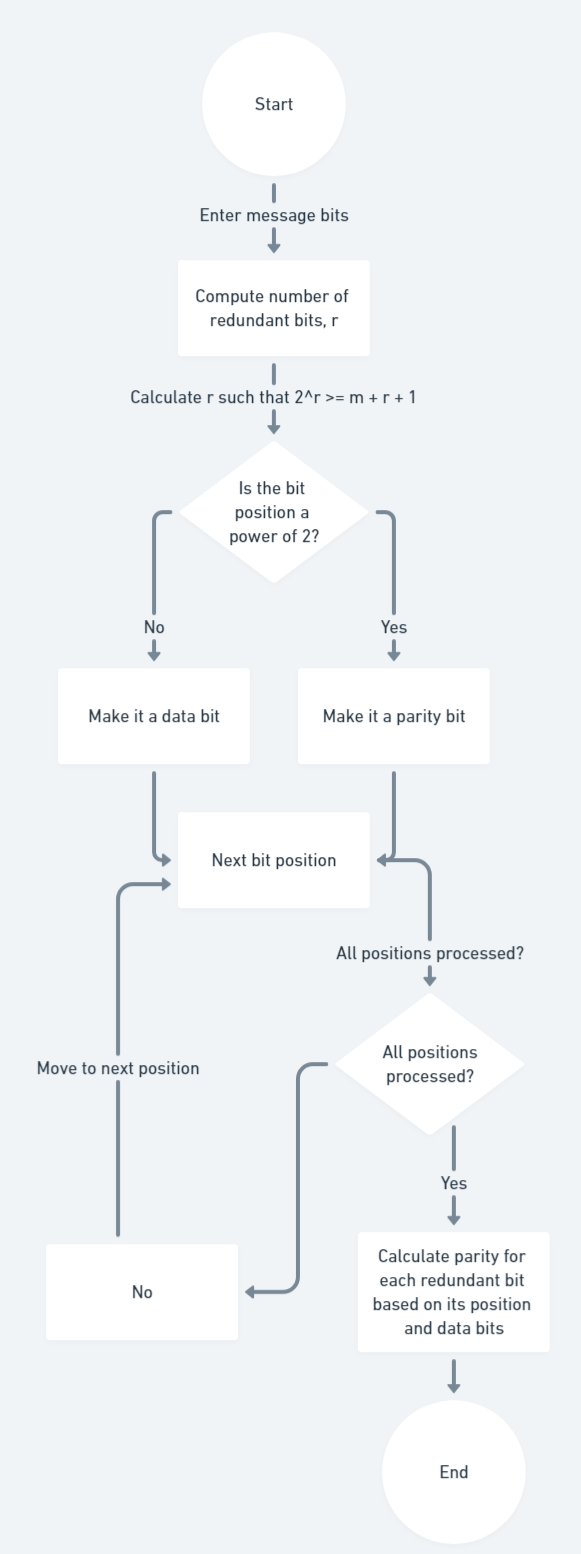
\includegraphics[scale=0.545]{encoding.png} 
       &
       

        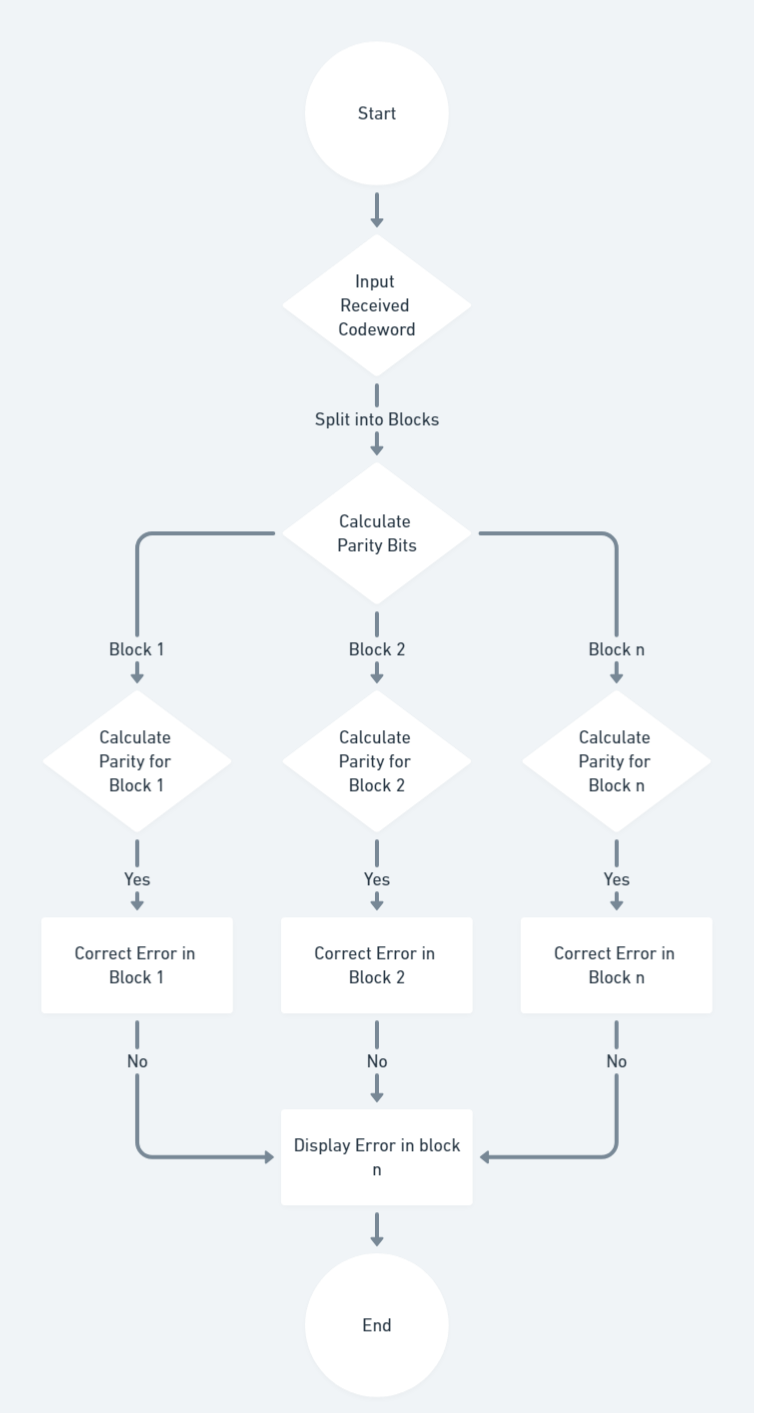
\includegraphics[scale=0.6]{decoding.png}
  



\end{tabular}

% \begin{minipage}{0.45\textwidth}
%     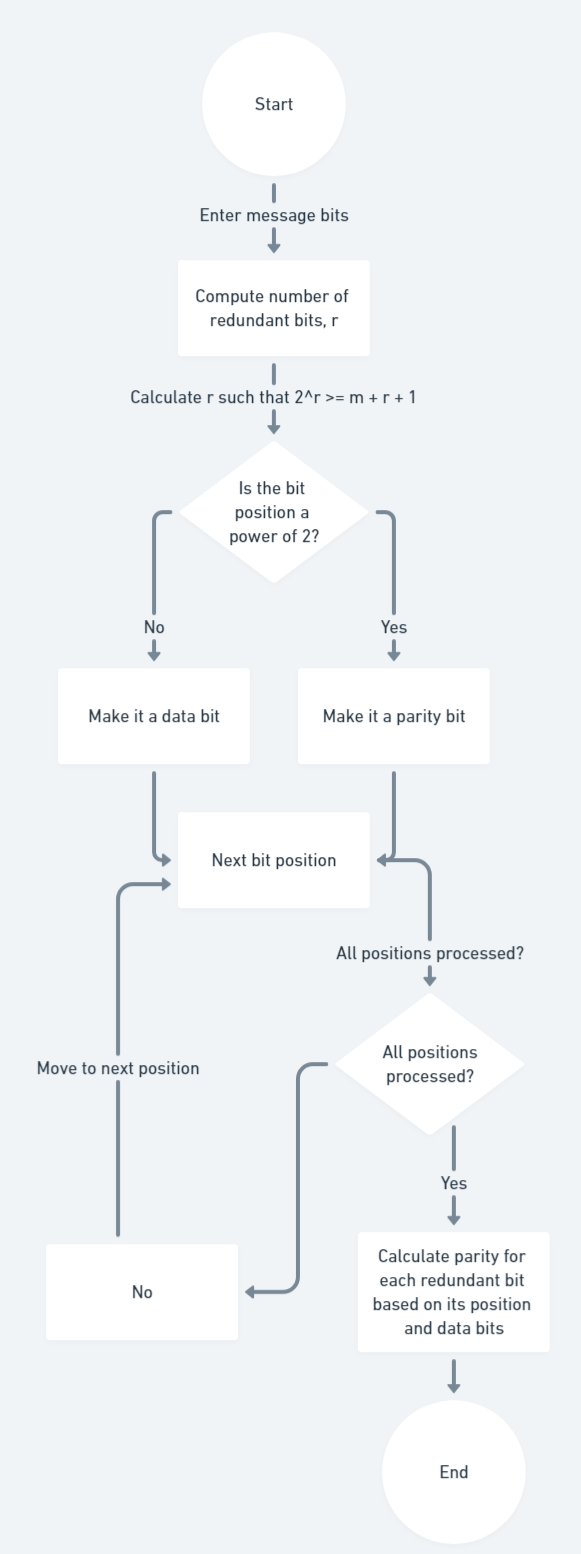
\includegraphics[scale=0.5]{encoding.png}
   
% \end{minipage}
% \hfill
% \begin{minipage}{0.45\textwidth}
%     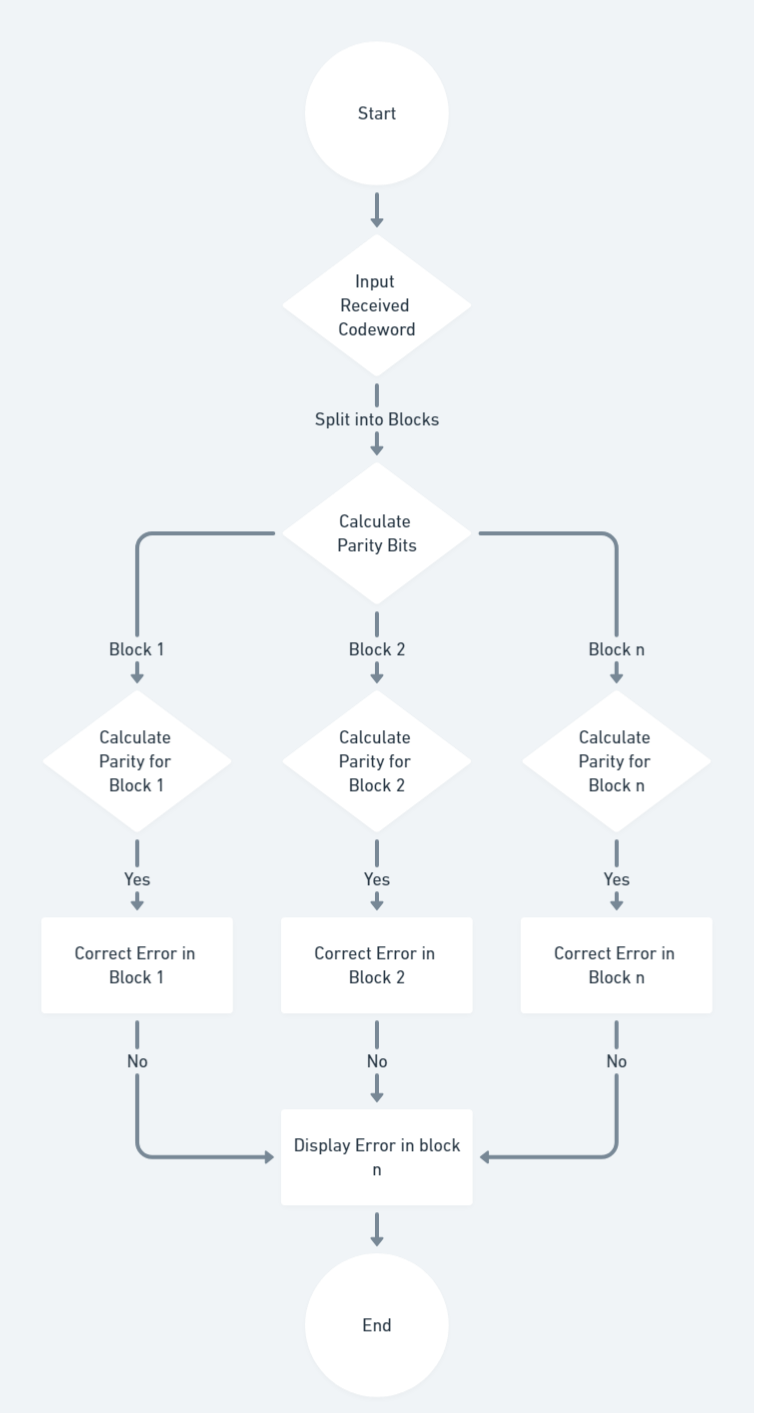
\includegraphics[scale=0.5]{decoding.png}
   
% \end{minipage}





 %   \subsection{Encoding Function}

 %       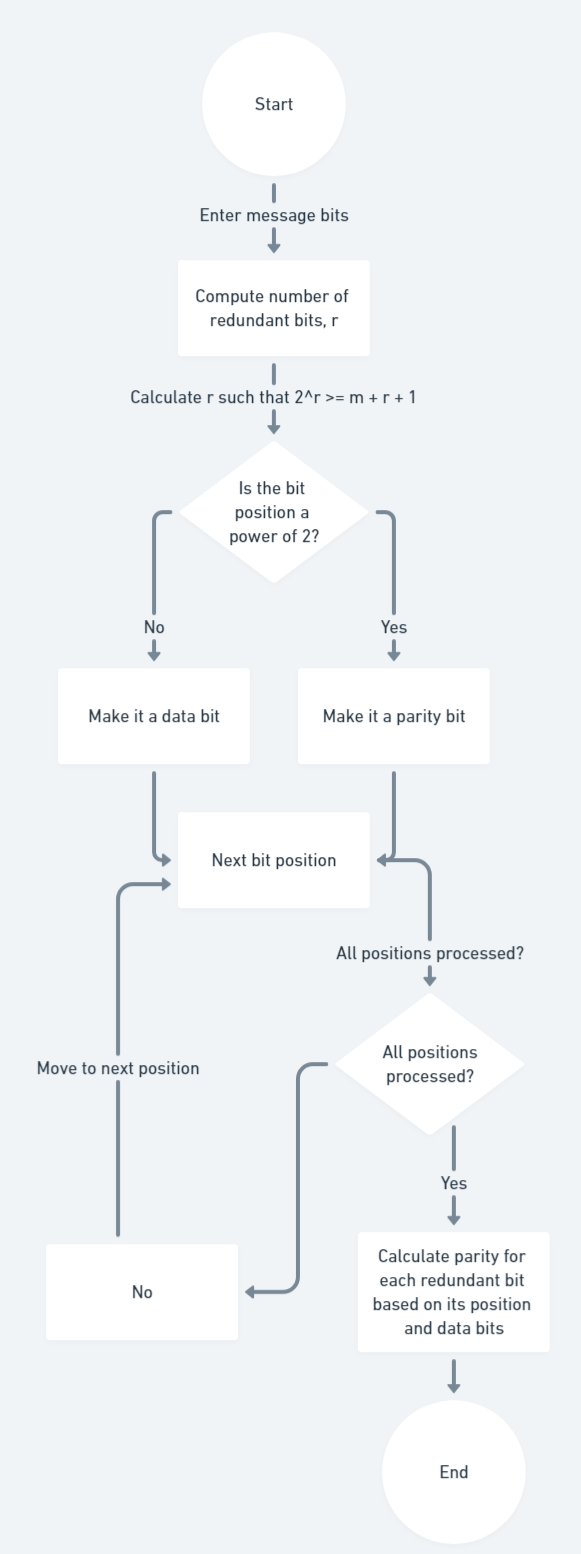
\includegraphics[width=0.3\linewidth]{encoding.png}
 
    
 % \subsection{Decoding Function}

 %    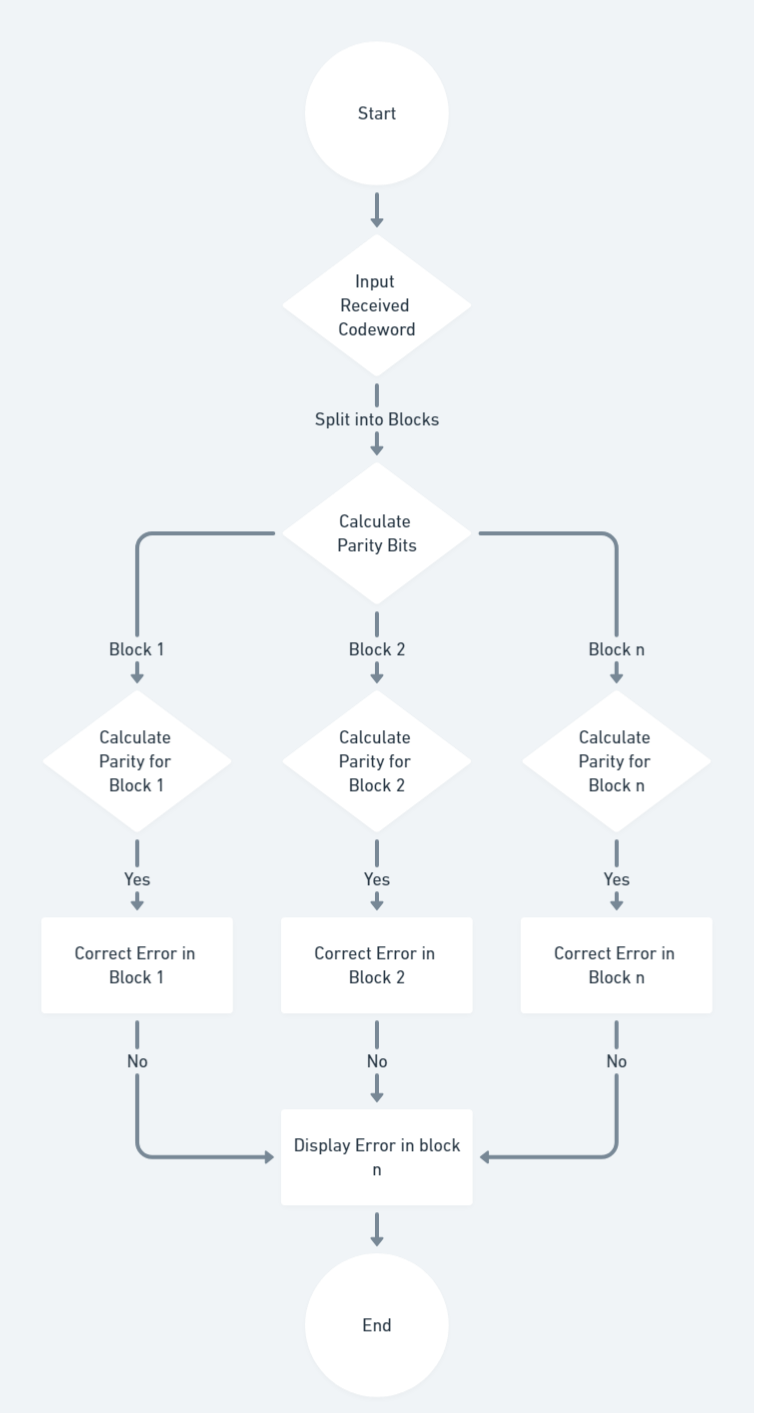
\includegraphics[width=0.5\linewidth]{decoding.png}


\section{OBJECTIVE-III : Implementing on Microprocessor}
Implement the Hamming (12,8) code encoding and decoding on a microprocessor, such as an Arduino. This implementation will allow real-time error detection and correction in data transmitted between devices.
\begin{enumerate}
    \item {Setting Up the Microprocessor}
        \begin{itemize}
        \item Use an Arduino (or similar micro controller) to send and receive data.
        \item Prepare two Arduino boards if you want to simulate the transmission of encoded data between devices.
        \item Connect the Arduinos via Serial or I2C communication, which allows them to send and receive data reliably.
        \end{itemize}
    \item{Programming the Encoder and Decoder}
    \begin{itemize}
        \item Write functions to encode 8-bit data into a 12-bit Hamming code.
        \item Write functions to decode the 12-bit Hamming code back into 8-bit data and correct single-bit errors if necessary.
        \item Store these functions in header files (\texttt{HammingEncoder.h} and \texttt{HammingDecoder.h}) for modularity and re-usability.
    \end{itemize}
    \item {Integrating the Hamming Encoder and Decoder Code}
    \begin{itemize}
    \item Import the encoder and decoder header files into your Arduino sketch.
    \item Designate one Arduino as the \textbf{transmitter} (encoding and sending data) and the other as the \textbf{receiver} (decoding and error-checking the received data).
    \end{itemize}
\end{enumerate}
\textbf {Tools for Hamming Code Implementation on an Arduino}

\begin{tabular}{|l|p{10cm}|}
\hline
\textbf{Tool} & \textbf{Description} \\
\hline
Arduino Board & The microcontroller board ie, Arduino nano using ATmega32P used for coding and testing the Hamming Code implementation. \\
\hline
Arduino IDE & Software used to write, compile, and upload code to the Arduino board. It provides an environment for developing Hamming code logic in C/C++. \\
\hline
Breadboard & Used for building and testing the circuit without soldering, connecting the Arduino pins with peripherals like LEDs and switches. \\
\hline
Jumper Wires & Used to make connections between the Arduino, breadboard, and other components in the circuit. \\
\hline
LEDs & Can be used as output indicators for testing Hamming code output such as error detection/correction results. \\
\hline
Resistors & Typically used with LEDs to limit current and protect components during testing and debugging. \\
\hline
Oscilloscope & A device used to observe and analyze the electrical signals in the circuit, which is helpful for debugging timing and signal integrity issues. \\
\hline
PS/2 Keyboard & A peripheral device that can be used for input testing and interfacing with the Arduino to send data streams that may require Hamming code error checking. \\
\hline
\end{tabular}







\pagebreak

\section{Methodology}
 \subsection{Thought Train Mapping}
    \begin{figure*}[!ht]
    \centering
    
    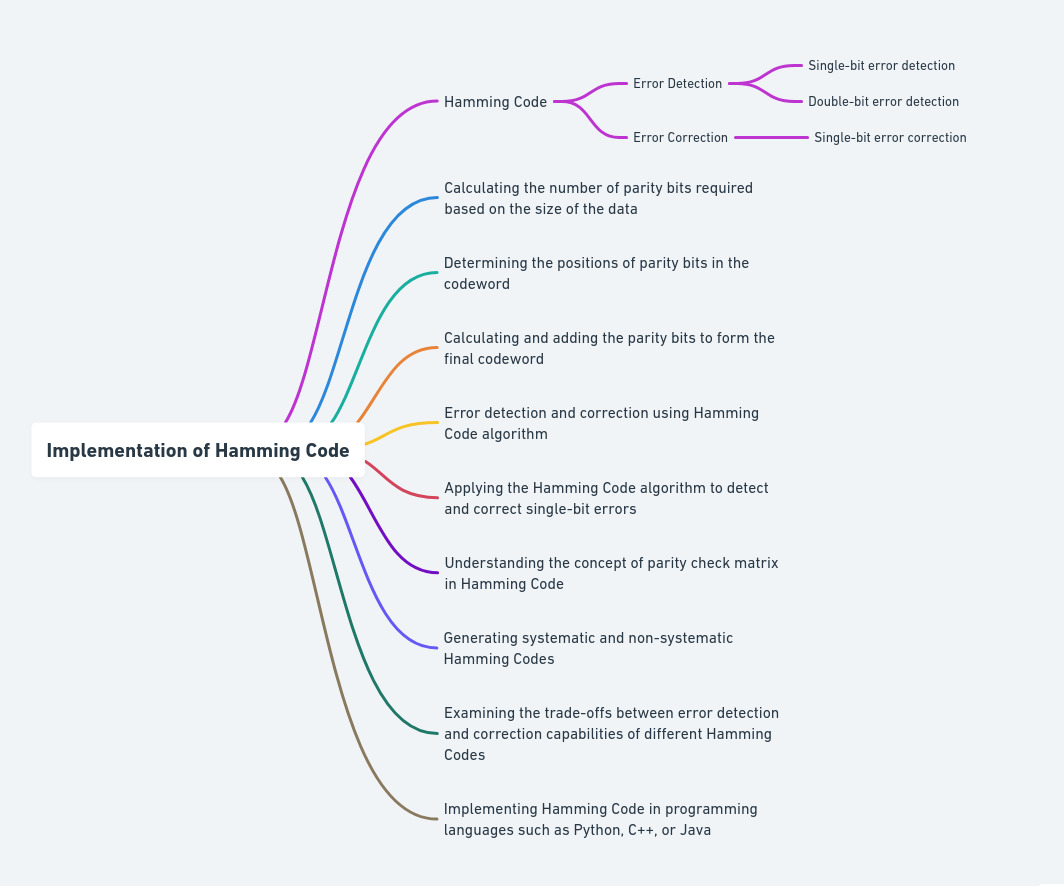
\includegraphics[width=20cm, height=10cm, keepaspectratio]{figures/flow1.jpeg}      
    
    \caption{Methodology Mindmap}
    \label{fig:fig2}
\end{figure*}
 \subsection{System design Mapping}
    \begin{figure*}[!ht]
    \centering
    
    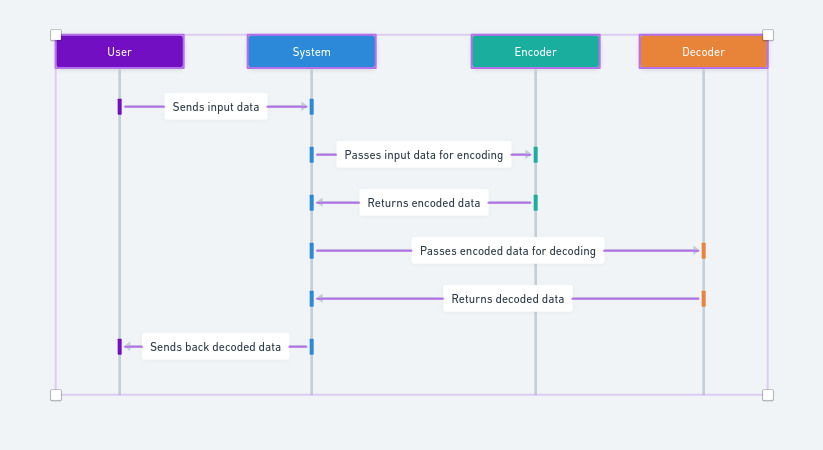
\includegraphics[width=14cm, height=8cm, keepaspectratio]{figures/system_design.jpeg}      
    
    \caption{Algorithim Sequence flow}
    \label{fig:fig3}
\end{figure*}


    
     
\section{Conclusions and Scope for Future Works}
Key findings of Hamming code implementation include:
\begin{itemize}
    \item \textbf{Error Detection and Correction Capability:} Hamming codes detect and correct single-bit errors, which enhances communication system reliability.
    \item \textbf{Low Complexity:} The encoding and decoding processes are computationally lightweight, suitable for real-time applications.
    \item \textbf{Hardware Efficiency:} Hamming codes can be effectively implemented in both software and hardware, including FPGA and ASIC designs.
\end{itemize}

% \textbf{Practical Implications}

% The practical implications of implementing Hamming code are extensive. In modern systems, the ability to ensure data reliability is essential, and Hamming code provides a balance between complexity and error-correction capability. Key applications include:
% \begin{itemize}
 

% \item {Communication Systems}
% Hamming codes are commonly used in communication protocols to detect and correct errors in data packets. This reduces retransmission, leading to faster and more reliable data transfers.

% \item {Memory Systems}
% In computer memory systems such as RAM and cache memory, Hamming code is used for error correction to ensure data integrity during read and write operations. ECC (Error-Correcting Code) memory uses Hamming codes to automatically correct errors without user intervention.

% \item {Storage Devices}
% Hamming codes are implemented in storage devices like hard drives, SSDs, and data storage systems to maintain data integrity, especially in the presence of noise or wear-related errors.
% \end{itemize}

\textbf{Scope for Future Work}

While Hamming codes provide a strong foundation for error detection and correction, further enhancements can extend their capabilities for evolving applications. Future work can focus on the following aspects:
\begin{itemize}

\item {Hardware Optimization}

Optimizing the hardware implementation of Hamming code, including faster encoding and decoding circuits, can benefit real-time communication and memory systems. This involves reducing power consumption, increasing speed, and enhancing scalability.

\item {Integration with Modern Protocols}

As communication protocols continue to evolve, integrating Hamming codes into modern network and communication standards, including wireless networks, 5G systems, and IoT applications.

\item {Quantum Error Correction}

Exploring the application of Hamming code principles in quantum computing environments, where quantum error correction is essential, can open new research directions and lead to novel hybrid quantum-classical solutions.
\end{itemize}
In conclusion, Hamming code remains a fundamental approach for error detection and correction. Continued research and development can expand its applications, making it more relevant for emerging technologies and critical communication systems.
    
%\bibliographystyle{plain}
\bibliographystyle{IEEEtran}
\bibliography{references}

\end{document}
